\chapter{研究方法}
\fontsize{12pt}{18pt}\selectfont

% ------------------------- 3.0 ------------------------- %
% 研究目的;研究假設;研究方法
本研究目的是透過最佳化方法估計肌肉參數,省去醫療器材量測之高成本,藉以生成個人化模型,
應用於復健規劃、運動訓練與輔具設計等領域。本研究假設為已知一肌肉骨骼模型,該模型除了欲評估之肌肉參數外,
其餘幾何特徵、肌肉參數等資訊皆為已知,而其可透過 OpenSim 軟體來執行任何模擬。研究方法主要分為三大主軸,
介紹如下:
\begin{itemize}
    \item \textbf{主軸一:敏感度分析}
    \\ 透過擾動肌肉參數,來計算出任務與參數間之敏感度,其指標是藉由預測任務之誤差來表示。
       敏感度高意味著該肌肉和該任務具有高相關性,其結果提供最佳化與模型驗證之任務挑選的參考依據。
    \item \textbf{主軸二:多運動軌跡預測最佳化}
    \\ 從敏感度分析挑選數個適當任務作為輸入,並將多運動軌跡預測任務之平均預測誤差視作目標函數,
       藉由最佳化方法最小化平均預測誤差,以此估計出最佳模型之肌肉參數。   
    \item \textbf{主軸三:模型驗證}
    \\ 從敏感度分析挑選適當任務作為輸入,指定最佳模型完成並檢視其預測誤差,
       確認該模型是否於其它任務仍具有低誤差表現,以此驗證模型正確性。
\end{itemize}

% 研究流程圖 + 說明
本研究之流程圖如圖 所示,首先輸入標準模型和分析參數來執行敏感度分析,
藉由全因子實驗設計法來評估出所有任務之敏感度指標,接下來挑選適合的組合集作為最佳化之評估任務,
以生成最佳模型,最終透過高敏感度任務進行模型驗證,來評估最佳模型之正確性。
若於模型驗證階段成功,代表評估正確,並結束程式執行;若於模型驗證階段失敗,則返回至最佳化步驟重新評估;
若模型驗證失敗次數過多,則返回至敏感度分析流程,重新挑選合適的評估任務。
程式碼將發布於 https://github.com/solab-ntu/MuscleParamEstimation 該網址中,執行細節可檢視程式碼中的註解說明。

\clearpage

% ------------------------- 3.1 ------------------------- %
\section{系統架設與實驗環境}
% 系統架設;實驗環境

\subsection{系統架設}
% 系統架設介紹
123123
\subsubsection{硬體-相機擺放}
% 硬體介紹;相機擺放
123123
\subsubsection{軟體-xsens}
% 軟體介紹;xsens
123123

\subsection{實驗環境}
% 實驗環境介紹
123123

% ------------------------- 3.2 ------------------------- %
\section{資料前處理}
% 資料前處理介紹
利用章節 3.1 介紹的系統蒐集完實驗資料後,接下來將進行資料前處理,以利後續進行感測器融合。
資料前處理分為人體骨架建立、時間軸對齊、座標系轉換三個部分,將於本章節進行討論。

\subsection{人體骨架建立}
% 人體骨架建立介紹
在文獻~\cite{zhang2020fusing} 中,作者使用 Vicon 系統所提供的骨架資料,
並以其為基礎,進行 IMU 計算;但是在非實驗室的環境中無法使用 Vicon 進行量測,進而取得骨架資料。
因此本研究透過 pose2sim~\cite{Pagnon_2021_Robustness}~\cite{Pagnon_2022_Accuracy}~\cite{Pagnon_2022_JOSS}提出之方法,
使用影像辨識技術辨識每一視角中人體的關節點位置,並利用相機校正技術建立出關節在空間中的位置,以此方式建立人體骨架,
後續利用 total capture dataset 提供的 Vicon 資料,進行影像辨識與三角化結果與 Vicon 資料的比對,以驗證此方法的可行性。

\subsubsection{建立方法}
% 影像辨識
% 這邊好像跟第四章的4.1.1有點重複,如果這邊和4.1都要留的話可能就要把下一節的結果與驗證搬到4.1那邊
% 這邊就只要簡單介紹一下方法就好,然後這邊可以應該可以把為何要選 openpose 不選 mediapipe 也寫上去
% 只是這樣的話就要想一下4.1.2的實驗執行要怎麼寫(不然如果真的想不到可能就要刪掉實驗執行這塊,畢竟也只是 run 而已),
% 4.1.1的應該可以寫用了哪些數據
本方法流程如圖~\ref{ch3_fig_skeleton_flow} 所示。
首先,使用 openpose~\cite{8765346}~\cite{wei2016cpm}~\cite{simon2017hand}~\cite{cao2017realtime}
影像辨識技術辨識每一視角中人體的關節點位置,辨識結果如圖~\ref{ch3_fig_openpose_result} 所示;
接著,利用棋盤格方法之相機校正技術計算出各個相機的內部參數及外部參數;
再來,利用方才相機校正之結果,經由三角化計算建立出關節在空間中的位置,並使用距離公式計算每一關節之間的距離;
最後,基於 total capture dataset 提供之 vicon 骨架,利用計算出的距離進行骨架伸縮,
得到與受試者四肢、身高相似之骨架,如圖\ref{}。
\begin{figure}[!ht]
   \centering
   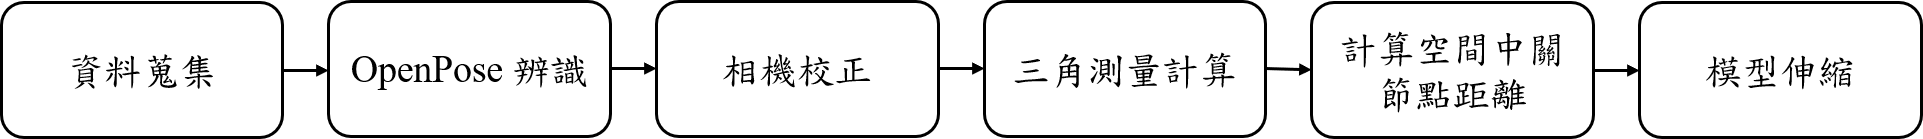
\includegraphics[width=8cm]{figure/ch3_fig_skeleton_flow.png}
    \caption[骨架建立流程圖]{骨架建立流程圖}
    \label{ch3_fig_skeleton_flow}
\end{figure}

\begin{figure}[!ht]
   \centering
   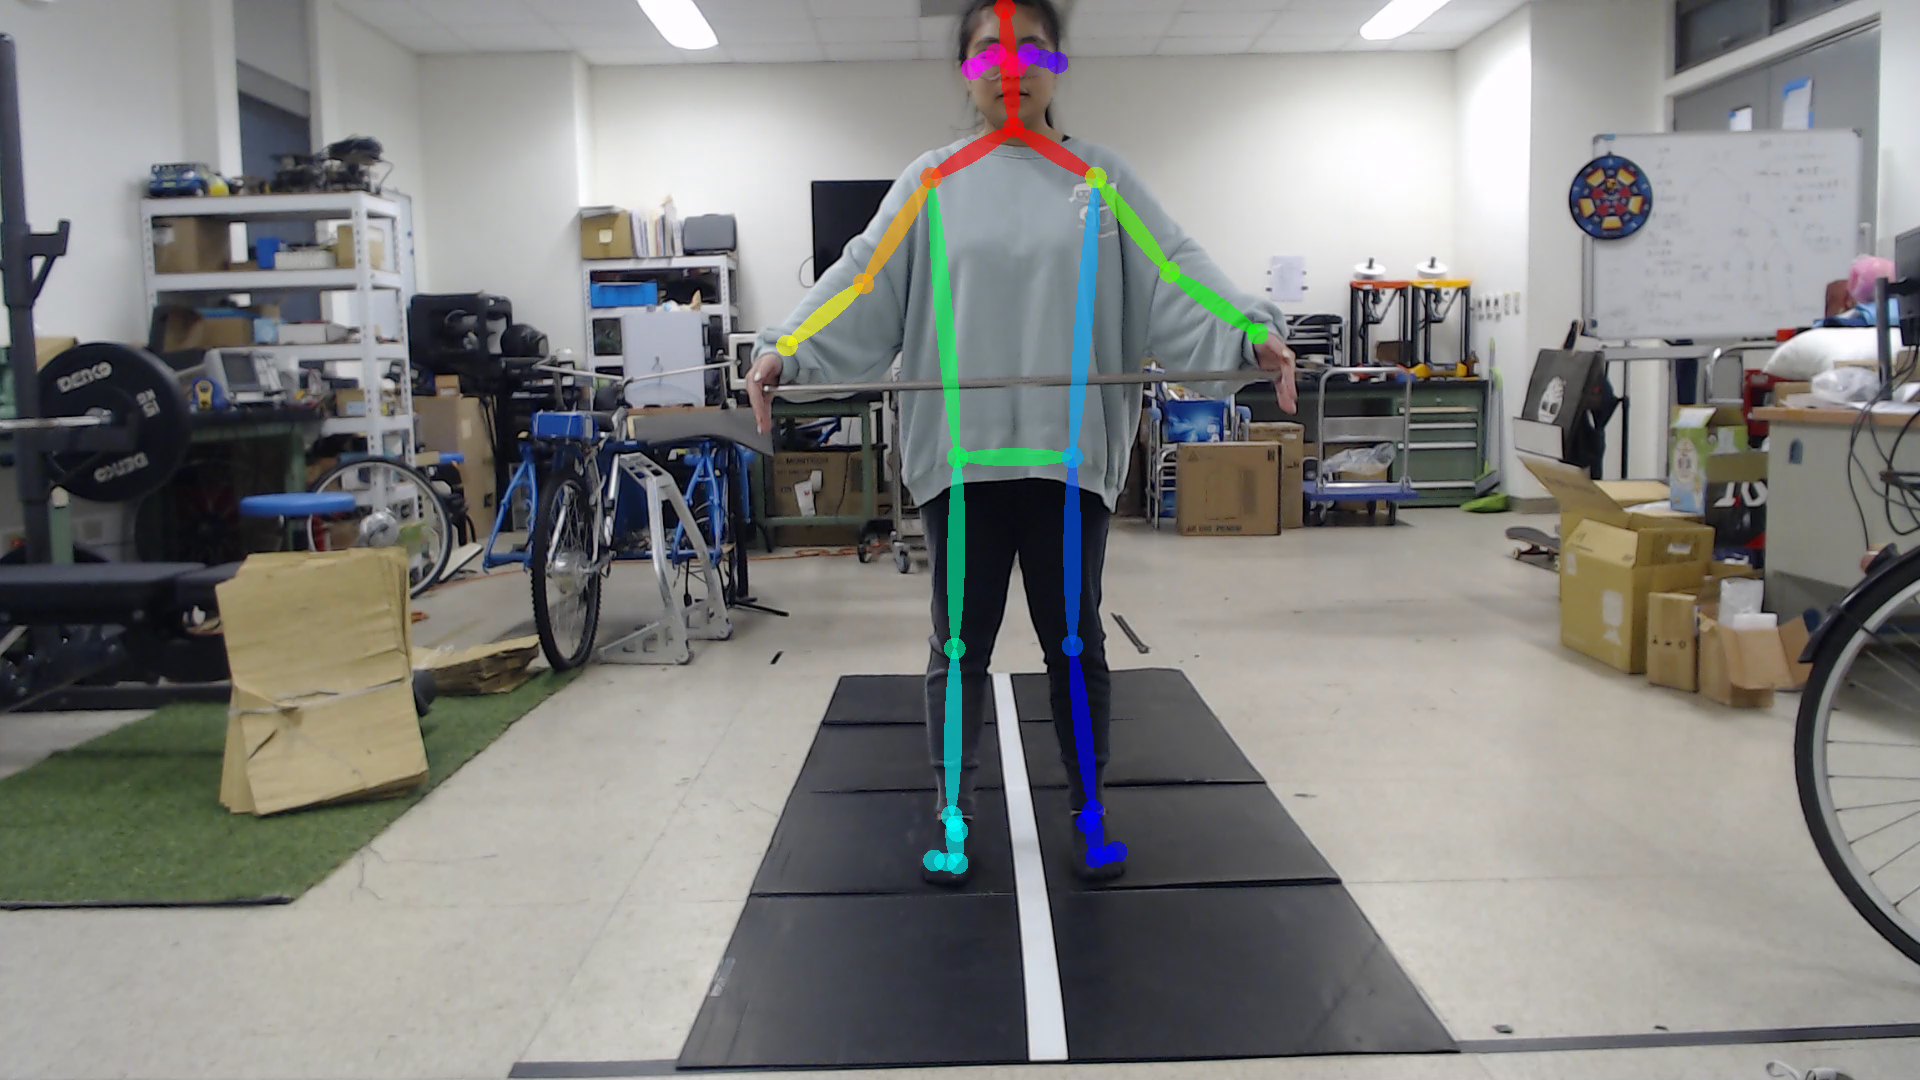
\includegraphics[width=8cm]{figure/ch3_fig_openpose_result.png}
    \caption[openpose 辨識結果]{openpose 辨識結果}
    \label{ch3_fig_openpose_result}
\end{figure}
% 用 minipage 的方法加上自己建立的骨架圖片

\subsection{時間軸對齊}
% 時間軸對齊介紹
拍手及加速度判斷

\subsection{座標系轉換}
% 座標系轉換介紹
% 似乎要cite一下這個方程式的來源,可是我也沒有提到這個方程式
在人體量測領域中,每一量測方法都有其固有且常用之座標系,
因此在進行感測器融合時,必須將各感測器之座標系轉換至同一座標系,以方便後續感測器融合計算。
本研究共會涉及四種座標系,分別為骨骼座標系,IMU local 座標系,IMU global 座標系,全域座標系。
其中,骨骼座標系以 total capture dataset 提供之 Vicon 骨架為基礎,如圖~\ref{ch3_fig_skeleton_frame}所示,
其 +x、+y、+z 方向分別為向右(red)、向後(green)、向下(blue);
IMU local 座標系即為感測器座標系,以感測器本身為原點,
於 Xsens 中,定義其 x 軸為長邊之延伸方向,y 軸為短邊之延伸方向,z 軸則沿最大平面之法向,
如圖~\ref{ch3_fig_imu_frame} 所示;
IMU global 座標系則以 x 軸指向正東,y 軸指向正北,z 軸指向天頂為正;
% 全域座標系還不知道怎麼定義QQ
\begin{figure}[!ht]
   \centering
   \begin{minipage}{.5\textwidth}
     \centering
     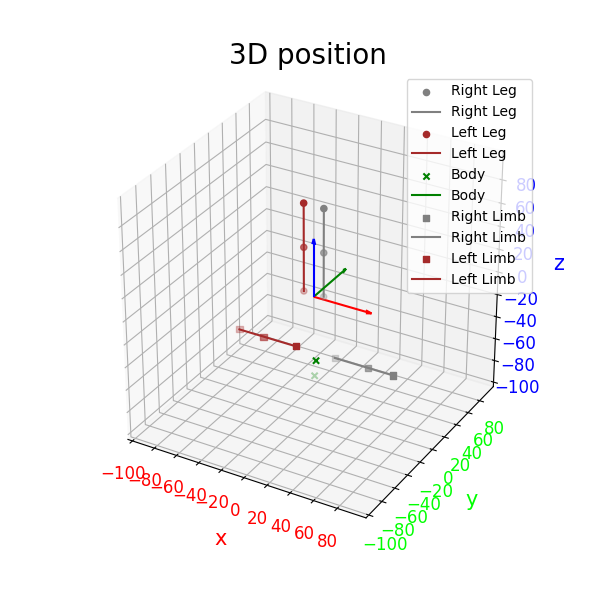
\includegraphics[width=.8\linewidth]{figure/ch3_fig_skeleton_frame.png}
     \caption[骨骼座標系定義]{骨骼座標系定義}
     \label{ch3_fig_skeleton_frame}
   \end{minipage}%
   \begin{minipage}{.5\textwidth}
     \centering
     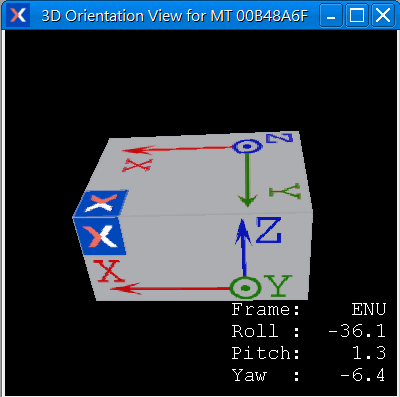
\includegraphics[width=.8\linewidth]{figure/ch3_fig_imu_frame.png}
     \caption[IMU local 座標系定義]{IMU local 座標系定義}
     \label{ch3_fig_imu_frame}
   \end{minipage}
\end{figure}

\subsubsection{IMU - 全域座標旋轉矩陣計算}
% IMU - 全域座標轉換矩陣計算介紹
$R_{ig}$

\subsubsection{IMU - 骨骼座標旋轉矩陣計算}
% IMU - 骨骼座標轉換矩陣計算介紹
使用 IMU 進行肢體朝向量測時,由於 IMU 黏貼於肢體上的方向及位置可能會和骨骼定義之方向及位置有所偏差,
因此需使用 IMU - 骨骼座標旋轉矩陣,將位於 IMU local 座標系的量測數值轉換至骨骼座標系,
此矩陣($R_{ib}$)可經由 OpenSim~\cite{delp2007OpenSim}處理並進一步計算而得,其取得及計算方式如下。
首先,量測結束之 IMU 資料將透過 OpenSim 軟體進行處理,並取得 IMU 相對每一骨骼之相對位置及角度,
處理結果可經由 OpenSim 軟體可視化,如圖~\ref{ch3_fig_imu_ori} 所示。
此項數據紀錄於 OpenSim 輸出之 .osim 檔案的 <BodySet> 元素中,<BodySet> 以骨骼為單位,
其中包含之 <components> 則記錄一附著於該骨骼上之 IMU 的相對位置及角度,
<translation> 代表該 IMU 的原點相對於其附著之骨骼原點的平移,
<orientation> 則代表該 IMU 的坐標軸相對於其附著之骨骼坐標軸的旋轉。
因此若將 <translation> 數值更改為零,則可看到 IMU 原點與骨骼原點重合,如圖~\ref{ch3_fig_imu_tra},
而若將 <orientation> 數值更改為零,則可看到 IMU 坐標軸與骨骼坐標軸平行,如圖~\ref{ch3_fig_imu_rot}。
因此,從 .osim 檔案取得每一 IMU 相對於骨骼之相對位置及角度後,即可計算出 IMU - 骨骼座標四元數。
\begin{figure}[!ht]
   \centering
   \begin{minipage}{.3\textwidth}
     \centering
     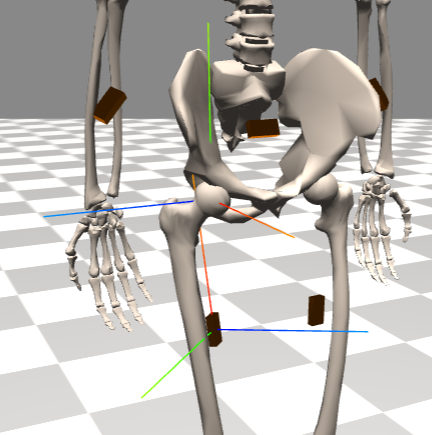
\includegraphics[width=.8\linewidth, height=.8\linewidth]{figure/ch3_fig_imu_ori.png}
     \caption[OpenSim 計算結果]{OpenSim 計算結果}
     \label{ch3_fig_imu_ori}
   \end{minipage}%
   \begin{minipage}{.3\textwidth}
     \centering
     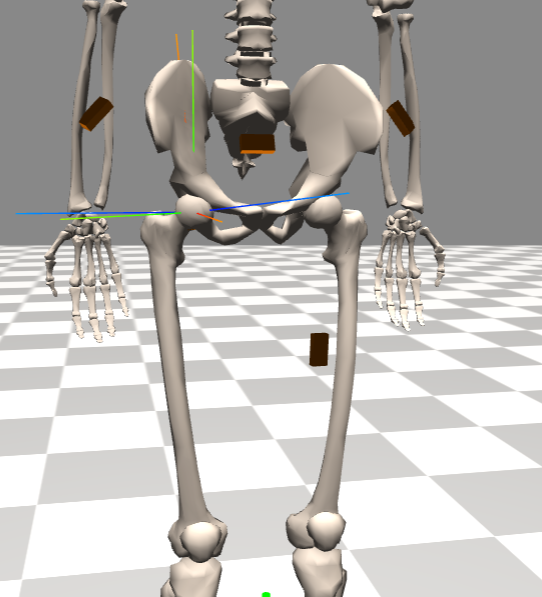
\includegraphics[width=.8\linewidth, height=.8\linewidth]{figure/ch3_fig_imu_tra.png}
     \caption[IMU 平移為零]{IMU 平移為零}
     \label{ch3_fig_imu_tra}
   \end{minipage}%
   \begin{minipage}{.3\textwidth}
      \centering
      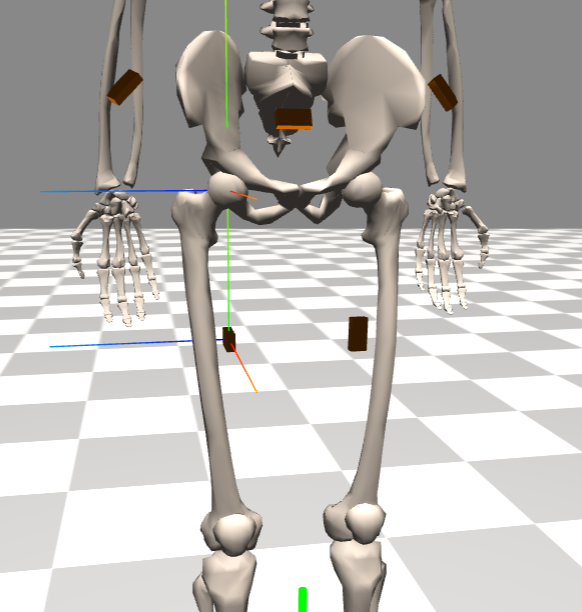
\includegraphics[width=.8\linewidth, height=.8\linewidth]{figure/ch3_fig_imu_rot.png}
      \caption[IMU 旋轉為零]{IMU 旋轉為零}
      \label{ch3_fig_imu_rot}
    \end{minipage}
\end{figure}

% ------------------------- 3.3 ------------------------- %
\section{探討減少相機數量的可行性及其擺放位置}
% 探討減少相機數量的可行性及其擺放位置介紹
total capture dataset~\cite{Trumble:BMVC:2017}提供之資料總共包含 8 台相機與 13 個 IMU 的 data,
而在文獻~\cite{zhang2020fusing}中,作者使用到 4 台相機及 8 個 IMU 的資料;
另外在 total capture dataset 發表的文獻~\cite{trumble2017total}中則有提及嘗試減少相機的硬體數量,準確度隨著相機數量的減少而下降,
因此本章節嘗試選擇相機數量與位置並進行感測器融合計算,
將得到的結果與 total capture dataset 提供的 Vicon 資料進行比對,計算 MPJPE,
藉此方式欲探討相機數量的減少對於動作捕捉的影響,並嘗試探討相機擺放位置的選擇。

\subsection{實驗方法-數量及位置選擇}
% 實驗方法介紹
% 目前的相機用量及擺放位置敘述,要 cite totalcapture 和 data fusion
從 total capture dataset 提供的影像資料可以觀察出其實驗環境為一個方形的空間,每一面牆面上方架設兩台相機,
四面牆共計八台相機,擺放位置如圖~\ref{ch3_fig_cameraset_totalcap} 所示。
\begin{figure}[!ht]
   \centering
   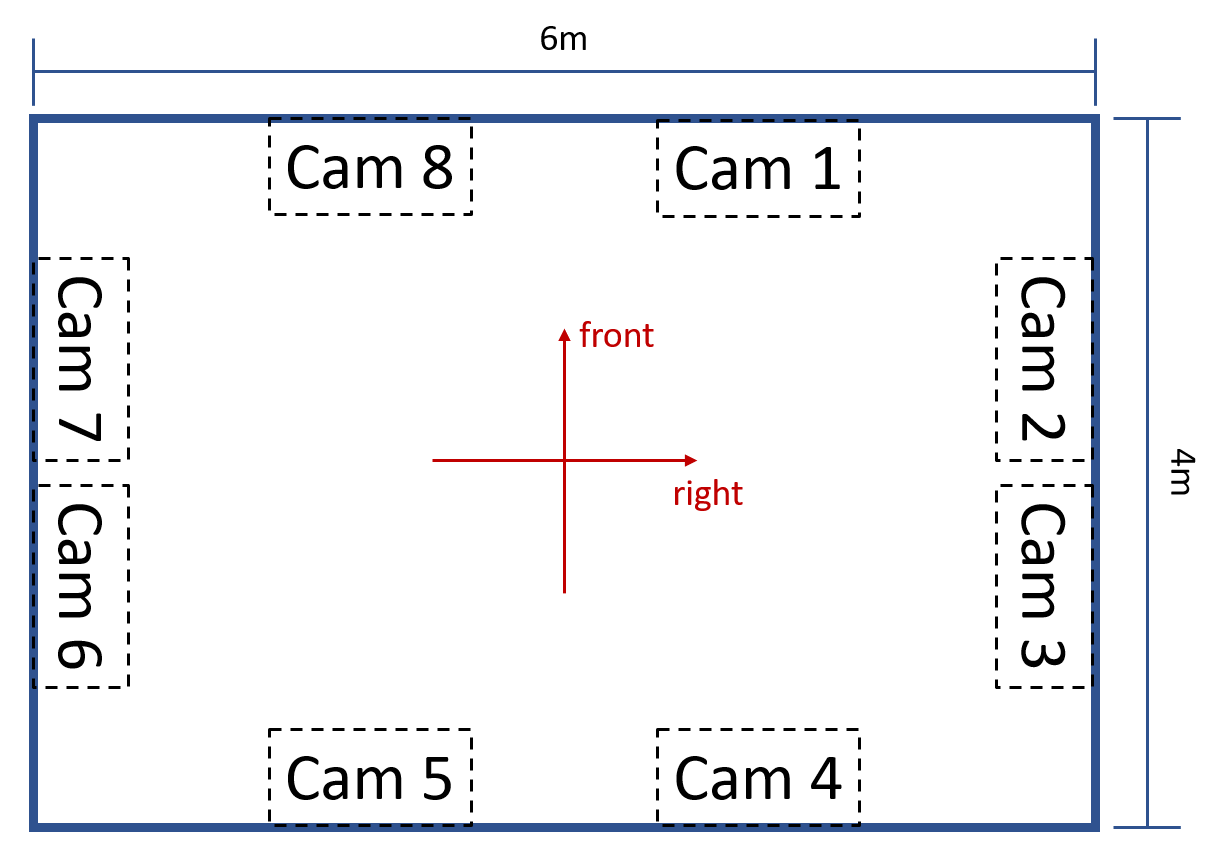
\includegraphics[width=8cm]{figure/ch3_fig_cameraset_totalcap.png}
    \caption[相機擺放位置]{相機擺放位置}
    \label{ch3_fig_cameraset_totalcap}
\end{figure}

\subsubsection{四台相機}
將圖~\ref{ch3_fig_cameraset_totalcap} 中的相機任選四台進行排列組合,共計有 70 種組合方式,每一種組合方式皆會產生一組 MPJPE,
結果如表~\ref{ch3_cameraset_4cam}所示,其中最佳組合方式為相機 1357,其 MPJPE 為 24.5789(mm);
而最差組合方式為相機 2567,其 MPJPE 為 38.9142(mm)。標準差為 3.6860(mm),平均值為 31.0114(mm)。
經由標準差可以知道四台相機組合的表現都相當穩定,無論如何選擇都不會有太大的影響。
\begin{table}[!ht]
   \caption[四台相機組合與其估計結果誤差]{四台相機組合與其估計結果誤差}
   \centering
   \label{ch3_cameraset_4cam}
   \setlength{\tabcolsep}{3pt}
   \renewcommand\arraystretch{1.5}
   \resizebox{\textwidth}{!}{
   \begin{tabular}{|
   >{\columncolor[HTML]{E7E6E6}}c |c|
   >{\columncolor[HTML]{E7E6E6}}c |c|
   >{\columncolor[HTML]{E7E6E6}}c |c|
   >{\columncolor[HTML]{E7E6E6}}c |c|
   >{\columncolor[HTML]{E7E6E6}}c |c|}
      \hline
      相機配置 & MPJPE & 相機配置 & MPJPE & 相機配置 & MPJPE & 相機配置 & MPJPE & 相機配置 & MPJPE \\
      \hline
      1234 & 30.9409 & 1235 & 28.8549 & 1236 & 30.3748 & 1237 & 28.8213 & 1238 & 31.1560 \\
      1245 & 33.1706 & 1246 & 31.5377 & 1247 & 32.1031 & 1248 & 33.6613 &            &         \\
      1256 & 34.5089 & 1257 & 34.6787 & 1258 & 35.2625 &            &         &            &         \\
      1267 & 31.7009 & 1268 & 33.0636 & 1278 & 34.6861 &            &         &            &         \\
      \hline
      1345 & 26.9753 & 1346 & 28.2925 & 1347 & 25.4715 & 1348 & 26.7584 &            &         \\
      1356 & 27.7651 & 1357 & 24.5789 & 1358 & 25.8578 &            &         &            &         \\
      1367 & 26.3845 & 1368 & 26.9445 & 1378 & 26.1466 &            &         &            &         \\
      \hline
      1456 & 29.9311 & 1457 & 26.6848 & 1458 & 27.9429 &            &         &            &         \\
      1467 & 26.8121 & 1468 & 27.5472 & 1478 & 27.1979 &            &         &            &         \\
      \hline
      1567 & 27.5824 & 1568 & 29.1892 & 1578 & 27.4552 & 1678 & 27.8378 &            &         \\
      \hline
      2345 & 34.0972 & 2346 & 36.5508 & 2347 & 36.7314 & 2348 & 33.7047 &            &         \\
      2356 & 35.6585 & 2357 & 36.3698 & 2358 & 30.8585 &            &         &            &         \\
      2367 & 36.8662 & 2368 & 32.6160 & 2378 & 34.8430 &            &         &            &         \\
      \hline
      2456 & 35.6440 & 2457 & 37.1359 & 2458 & 33.4067 &            &         &            &         \\
      2467 & 35.8266 & 2468 & 33.2654 & 2478 & 36.6081 &            &         &            &         \\
      2567 & 38.9142 & 2568 & 33.7187 & 2578 & 38.7211 & 2678 & 34.3506 &            &         \\
      \hline
      3456 & 32.4429 & 3457 & 27.7338 & 3458 & 27.6554 &            &         &            &         \\
      3467 & 31.0735 & 3468 & 29.9925 & 3478 & 27.9168 &            &         &            &         \\
      3567 & 29.2876 & 3568 & 28.3170 & 3578 & 26.8460 & 3678 & 29.4004 &            &         \\
      \hline
      4567 & 29.8717 & 4568 & 29.7963 & 4578 & 28.2055 & 4678 & 28.9104 & 5678 & 29.5824 \\
      \hline
   \end{tabular}}
\end{table}

\clearpage

\subsubsection{三台相機}
將圖~\ref{ch3_fig_cameraset_totalcap} 中的相機任選三台進行排列組合,共計有 56 種組合方式,每一種組合方式皆會產生一組 MPJPE,
結果如表~\ref{ch3_cameraset_3cam}所示,其中最佳組合方式為相機 137,其 MPJPE 為 27.1579(mm);
而最差組合方式為相機 257,其 MPJPE 為 82.8158(mm)。標準差為 13.8423(mm),平均值為 42.9001(mm)。
經由標準差可以知道三台相機的組合相較四台相機來說表現相對較不穩定,
但只要位置恰當,僅用三台相機也可以有四台相機的表現水準。
\begin{table}[!ht]
   \caption[三台相機組合與其估計結果誤差]{三台相機組合與其估計結果誤差}
   \centering
   \label{ch3_cameraset_3cam}
   \setlength{\tabcolsep}{3pt}
   \renewcommand\arraystretch{1.5}
   \resizebox{\textwidth}{!}{
   \begin{tabular}{|
   >{\columncolor[HTML]{E7E6E6}}c |c|
   >{\columncolor[HTML]{E7E6E6}}c |c|
   >{\columncolor[HTML]{E7E6E6}}c |c|
   >{\columncolor[HTML]{E7E6E6}}c |c|
   >{\columncolor[HTML]{E7E6E6}}c |c|}
      \hline
      相機配置 & MPJPE & 相機配置 & MPJPE & 相機配置 & MPJPE & 相機配置 & MPJPE & 相機配置 & MPJPE \\
      \hline
      123 & 41.8538 & 124 & 43.2544 & 125 & 70.4747 & 126 & 41.7470 & 127 & 54.5721 \\
      128 & 46.7714 & & & & & & & & \\
      \hline
      134 & 30.9862 & 135 & 29.0275 & 136 & 33.6116 & 137 & 27.1579 & 138 & 29.9961 \\
      \hline
      145 & 34.4860 & 146 & 32.7227 & 147 & 29.9785 & 148 & 31.5573 & & \\
      \hline
      156 & 38.3802 & 157 & 33.2107 & 158 & 33.4297 & & & & \\
      \hline
      167 & 32.4098 & 168 & 33.4044 & 178 & 32.2636 & & & & \\
      \hline
      234 & 52.0193 & 235 & 76.4435 & 236 & 52.6657 & 237 & 65.5297 & 238 & 44.5936 \\
      \hline
      245 & 76.6047 & 246 & 42.4841 & 247 & 54.8719 & 248 & 45.2496 & & \\
      \hline
      256 & 74.8608 & 257 & 82.8158 & 258 & 62.4336 & & & & \\
      \hline
      267 & 58.7578 & 268 & 39.2619 & 278 & 62.7102 & & & & \\
      \hline
      345 & 35.9928 & 346 & 42.7418 & 347 & 35.2381 & 348 & 33.5695 & & \\
      \hline
      356 & 42.9933 & 357 & 35.1894 & 358 & 29.6995 & & & & \\
      \hline
      367 & 40.0411 & 368 & 35.8360 & 378 & 34.9221 & & & & \\
      \hline
      456 & 40.0658 & 457 & 37.2030 & 458 & 32.7289 & & & & \\
      \hline
      467 & 35.6906 & 468 & 33.8860 & 478 & 35.3151 & & & & \\
      \hline
      567 & 41.5287 & 568 & 34.8289 & 578 & 37.5083 & & & & \\
      \hline
      678 & 34.8273 & & & & & & & & \\
      \hline
   \end{tabular}}
\end{table}

\clearpage

\subsubsection{兩台相機}
將圖~\ref{ch3_fig_cameraset_totalcap} 中的相機任選兩台進行排列組合,共計有 28 種組合方式,每一種組合方式皆會產生一組 MPJPE,
結果如表~\ref{ch3_cameraset_2cam}所示,其中最佳組合方式為相機 18,其 MPJPE 為 46.9798(mm);
而最差組合方式為相機 25,其 MPJPE 為 300.1637(mm)。標準差為 61.7928(mm),平均值為 109.8694(mm)。
經由結果可以發現相機的擺放位置對估計結果影響甚鉅,若位置選擇得宜,估計結果將會相當準確,反之則會有較大的誤差。
\begin{table}[!ht]
   \caption[兩台相機組合與其估計結果誤差]{兩台相機組合與其估計結果誤差}
   \centering
   \label{ch3_cameraset_2cam}
   \setlength{\tabcolsep}{3pt}
   \renewcommand\arraystretch{1.5}
   \resizebox{\textwidth}{!}{
   \begin{tabular}{|
   >{\columncolor[HTML]{E7E6E6}}c |c|
   >{\columncolor[HTML]{E7E6E6}}c |c|
   >{\columncolor[HTML]{E7E6E6}}c |c|
   >{\columncolor[HTML]{E7E6E6}}c |c|}
      \hline
      相機配置 & MPJPE & 相機配置 & MPJPE & 相機配置 & MPJPE & 相機配置 & MPJPE \\
      \hline
      12 & 194.4957 & 13 & 81.9440 & 14 & 47.4927 & 15 & 76.7795 \\
      16 & 66.8653 & 17 & 58.7619 & 18 & 46.9798 & & \\
      \hline
      23 & 227.5722 & 24 & 182.6378 & 25 & 300.1637 & 26 & 183.0773 \\
      27 & 181.6520 & 28 & 145.2458 & & & &\\
      \hline
      34 & 99.3426 & 35 & 109.4178 & 36 & 92.7550 & 37 & 97.7435 \\
      38 & 81.3640 & & & & & &\\
      \hline
      45 & 87.4750 & 46 & 66.8800 & 47 & 67.4949 & 48 & 52.3318 \\
      \hline
      56 & 126.3387 & 57 & 95.1469 & 58 & 64.6374 & &\\
      \hline
      67 & 100.7632 & 68 & 63.7904 & & & &\\
      \hline
      78 & 77.1948 & & & & & &\\
      \hline
   \end{tabular}}
\end{table}

\clearpage

\subsubsection{一台相機}
將圖~\ref{ch3_fig_cameraset_totalcap} 中的相機任選一台進行估計,共計 8 種估計結果,每一結果皆會產生一組 MPJPE,
結果如表~\ref{ch3_cameraset_2cam}所示,可以發現無論選擇哪一個位置,其估計誤差皆超過 500 mm,
因此本研究認為只使用一台相機進行估計是不可行的,至少需使用兩台相機進行量測。
\begin{table}[!ht]
   \caption[一台相機組合與其估計結果誤差]{一台相機組合與其估計結果誤差}
   \centering
   \label{ch3_cameraset_1cam}
   \setlength{\tabcolsep}{3pt}
   \renewcommand\arraystretch{1.5}
   \resizebox{\textwidth}{!}{
   \begin{tabular}{|
   >{\columncolor[HTML]{E7E6E6}}c |c|
   >{\columncolor[HTML]{E7E6E6}}c |c|
   >{\columncolor[HTML]{E7E6E6}}c |c|
   >{\columncolor[HTML]{E7E6E6}}c |c|}
      \hline
      相機配置 & MPJPE & 相機配置 & MPJPE & 相機配置 & MPJPE & 相機配置 & MPJPE \\
      \hline
      1	& 514.76 & 2 & 782.01 & 3 & 611.84 & 4 & 520.97 \\
      5	& 653.96 & 6 & 573.41 & 7 & 599.78 & 8 & 542.36 \\
      \hline
   \end{tabular}}
\end{table}

\subsection{結果與討論}
% 結果介紹與討論
將一台相機到四台相機的組合估計結果繪製成圖~\ref{ch3_fig_1.2.3.4cam},可以發現四台相機的結果相較於三台相機來說比較穩定,
MPJPE 約都在 20~40 mm 左右,只是如果三台相機的配置適當的話,結果並不會比四台相機的結果差。
\begin{figure}[!ht]
   \centering
   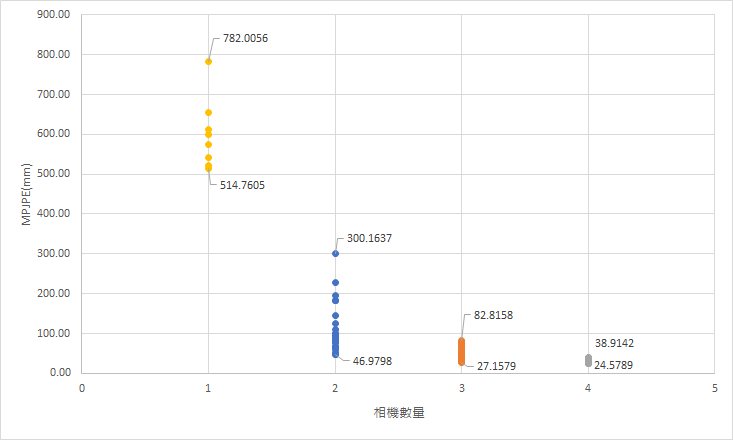
\includegraphics[width=12cm]{figure/ch3_fig_1.2.3.4cam.png}
   \caption[一台相機到四台相機的組合估計結果]{一台相機到四台相機的組合估計結果}
   \label{ch3_fig_1.2.3.4cam}
\end{figure}

另外列出每一相機數量的最佳表現及最差表現,如表~\ref{ch3_best_worst_camset},可以發現相機 1 皆有出現在最佳表現的結果中,而相機 2 皆有出現在最差表現的結果中,
因此推論相機 1 的位置較為適當。
\begin{table}[!ht]
   \caption[相機組合的最差及最佳表現]{相機組合的最差及最佳表現}
   \centering
   \label{ch3_best_worst_camset}
   \setlength{\tabcolsep}{3pt}
   \renewcommand\arraystretch{1.5}
   \begin{tabular}{c|c|c|c|c}
       & 1 cam & 2 cam & 3 cam & 4 cam \\ 
      \midrule[2pt]
      最差表現 & 2 & 25 & 257 & 2567 \\
      最佳表現 & 1 & 18 & 137 & 1357 \\
   \end{tabular}
\end{table}

\subsection{延伸討論}
% 延伸討論
由於目前~\cite{zhang2020fusing}取用四台相機,因此若欲減少相機使用數量勢必會往三台相機及兩台相機的配置進行考量,
因此以下將進一步比較三台相機及兩台相機的估計結果,並進行討論。

\subsubsection{方法}
將三台相機的估計結果依照兩台相機的配對進行平均,再與兩台相機的結果相減,以此方式觀察多一台相機的影響。
計算方式如算式~\ref{ch3_3camaveMin2cam}。
\begin{equation}
   \label{ch3_3camaveMin2cam}
   \text{差值} = \text{ave}(\text{MPJPE}_{3 \text{ cam}})-\text{MPJPE}_{2 \text{ cam}}
\end{equation}

\subsubsection{結果}
以下表~\ref{ch3_ave_3cam_vs_2cam} 交互相機 18 為例,即將 128、138、148、158、168、178 六組相機配對的估計結果進行平均,
得 MPJPE = 34.5704,再與直接用兩台相機進行融合估計得到的 MPJPE = 46.9798 相減,得 12.4094。
由下表~\ref{ch3_ave_3cam_vs_2cam} 可知,相機 1 及相機 8 的配對再加上第三台相機較不會有顯著的改善,
且前三種配對 (即配對 18、配對 14、配對 48)的改善皆都落在約 10~15 mm 左右,
所以可以推斷,相機 1、4、8 三個位置,隨意取其中兩者可能是較適合擺放相機的位置。
\begin{table}[!ht]
   \caption[兩台相機與三台相機平均之比較]{兩台相機與三台相機平均之比較}
   \centering
   \label{ch3_ave_3cam_vs_2cam}
   \setlength{\tabcolsep}{3pt}
   \renewcommand\arraystretch{1.5}
   \begin{tabular}{c|c|c|c}
      交互相機 & $ave(MPJPE_{3 cam})$ & $MPJPE_{2 cam}$ & 差 \\
      \midrule[2pt]
      18 & 34.5704 & 46.9798 & 12.4094 \\
      14 & 33.8308 & 47.4927 & 13.6619 \\
      48 & 35.3844 & 52.3318 & 16.9474 \\
      17 & 34.9321 & 58.7619 & 23.8298 \\ 
      58 & 38.4382 & 64.6374 & 26.1993 \\
      68 & 35.3408 & 63.7904 & 28.4496 \\
      46 & 37.9318 & 66.8800 & 28.9481 \\  
      47 & 38.0495 & 67.4949 & 29.4454 \\ 
      16 & 35.3793 & 66.8653 & 31.4860 \\ 
      15 & 39.8348 & 76.7795 & 36.9447 \\
      78 & 39.5911 & 77.1948 & 37.6037 \\
   \end{tabular}
\end{table}

另外,若希望 $MPJPE_{2 cam}$ 低於 80 mm,則從兩台相機的估計結果(表~\ref{ch3_cameraset_2cam})挑選出 $MPJPE_{2 cam}$ 低於 80 mm 的結果,
並計算每一相機的出現次數,則可得出如下表~\ref{ch3_cam_occurrence} 的結果,觀察下表也可發現相機 1、8 的出現次數最高,
其次為相機 4 ,因此也可推斷相機 1、4、8 三個位置可能是較適合擺放相機的位置。
\begin{table}[!ht]
   \caption[兩台相機估計結果之每台相機的出現次數]{兩台相機估計結果之每台相機的出現次數}
   \centering
   \label{ch3_cam_occurrence}
   \setlength{\tabcolsep}{3pt}
   \renewcommand\arraystretch{1.5}
   \begin{tabular}{c|c}
      相機 & 出現次數 \\
      \midrule[2pt]
      1 & 5 \\
      2 & 0 \\
      3 & 0 \\
      4 & 4 \\
      5 & 2 \\
      6 & 3 \\
      7 & 3 \\
      8 & 5 \\
   \end{tabular}
\end{table}

% ------------------------- 3.4 ------------------------- %
\section{結果可視化}
% 結果可視化介紹
還沒想到要寫甚麼

% ------------------------- 3.5 ------------------------- %
\section{小結}
% 本章架構
本章節首先介紹將會使用到的背景知識,像是透過希爾式肌肉模型來模擬肌肉,藉此理解肌肉的機械與生理特性,
而藉由 OpenSim 的協助,不但能快速建立肌肉骨骼模型,還可以執行正向動力學與肌肉計算控制等模擬,
且得到一個可信的結果,接下來介紹本研究的核心模擬——運動軌跡預測任務,後續的敏感度分析、最佳化過程與模型驗證,
皆是以預測任務為基礎來延伸,透過預測任務來檢視模型的表現,亦即預測誤差。
本研究透過敏感度分析來得知肌肉與任務之間的關係,藉此挑選合適的任務集作為參數評估輸入,
搭配最佳化演算法來進行參數估計,其中多組預測任務具有讓目標函數更加明確的功用,避免參數不具識別性的原因,
掉入至局部最小值結果當中,最終透過間接方法來驗證模型的正確性。

% 應用
該研究方法之應用可分為兩種討輪,第一是模擬研究,即為本研究使用之方法,透過純模擬研究來檢視該方法的可行性,
優點是其具有明確答案可供參考,且無需考慮量測造成的不確定性,在進入到實際應用前,也必須先確認模擬研究是可執行的;
第二種則是實際應用,其可透過 EMG 與動作捕捉系統來達成,藉由 EMG 量測肌肉訊號作為輸入,
動作捕捉系統量測運動軌跡作為輸出之結果比較,兩者結合並搭配本研究之最佳化方法,即可達成肌肉之參數估計,
但存在龐大的量測不確定性情況下,由於微小的軌跡偏離,即會造成肌肉參數的變動與抗衡,
縱使估計出肌肉參數,其結果之正確性仍有待商榷,因此於現今之科技發展,要達成實際應用仍有一段距離。

% 下一章節
本章節主要介紹論文之研究方法,下章節會以實際模型與動作進行討論,藉由上方所提及之方法與流程,
針對模型進行肌肉參數評估的前置作業與套用說明。

\clearpage